%!TEX program = xelatex
\documentclass[a4paper,12pt]{article}
	\linespread{1.3}

\usepackage{geometry} 
	\geometry{left=3cm}
	\geometry{right=1cm}
	\geometry{top=2cm}
	\geometry{bottom=2cm}

\usepackage[fleqn]{amsmath}
\usepackage{unicode-math}
\usepackage{multirow}

\usepackage[english,russian]{babel}
\usepackage{indentfirst}

\usepackage{graphicx}
	\let\ORIincludegraphics\includegraphics
	%\renewcommand{\includegraphics}[2][]{\ORIincludegraphics[scale=0.7,#1]{#2}}

\usepackage{fontspec}
	\defaultfontfeatures{Scale=MatchLowercase}
	\setmainfont[Mapping=tex-text]{Minion Pro}
	\setmonofont{Menlo}

\usepackage{listings}
	\lstset{
		extendedchars=true,
		showspaces=false,
		showtabs=false,
		breaklines=true,
		showstringspaces=false,
		breakatwhitespace=true,
		basicstyle=\ttfamily\small
	}
\usepackage{verbatim}

\usepackage[dvipsnames]{xcolor}

\usepackage{tabularx,booktabs}

\usepackage[nooneline]{caption}
	\captionsetup{textformat=period, figurename=Рисунок}
	\captionsetup[table]{justification=raggedright}
	\captionsetup[figure]{justification=centering} 
	\DeclareCaptionLabelSeparator{tier}{ --- }
	\captionsetup{labelsep=tier}

\usepackage{subcaption}
	\DeclareCaptionSubType*{figure}
	\renewcommand{\thesubfigure}{\asbuk{subfigure}}

\usepackage{floatrow}
	\floatsetup[table]{capposition=top}

%\usepackage{pdflscape}
\usepackage{calc}
\usepackage{enumitem}
\makeatletter
    \AddEnumerateCounter{\asbuk}{\@asbuk}{м)}
	\makeatother
	\setlist{nolistsep}
	\renewcommand{\labelitemi}{--}
	\renewcommand{\labelitemii}{--}
	\renewcommand{\labelitemiii}{--}
	\renewcommand{\labelenumi}{\asbuk{enumi})}
	\renewcommand{\labelenumii}{\arabic{enumii})}
	\renewcommand{\labelenumiii}{\asbuk{enumiii})}

\usepackage{tikz}
	\usetikzlibrary{arrows}

\usepackage{titlesec}
	\titleformat{\chapter}[display]
	    {\filcenter}
	    {}
	    {8pt}
	    {\bfseries}{}

	\titleformat{\section}
	    {\normalsize\bfseries}
	    {\thesection}
	    {1em}{}
 
	\titleformat{\subsection}
	    {\normalsize\bfseries}
	    {\thesubsection}
	    {1em}{}

    \titlespacing*{\chapter}{0pt}{-30pt}{8pt}
	\titlespacing*{\section}{\parindent}{*4}{*4}
	\titlespacing*{\subsection}{\parindent}{*4}{*4}
	\titlespacing*{\subsubsection}{\parindent}{*4}{*4}

\usepackage{tocloft}
	\renewcommand{\cfttoctitlefont}{\hspace{0.38\textwidth} \bfseries\MakeUppercase}

\usepackage{titletoc}
	\dottedcontents{section}[1em]{}{1em}{1pc}

\addto\captionsrussian{% Replace "english" with the language you use
  \renewcommand{\contentsname}%
    {СОДЕРЖАНИЕ}%
}


\newcommand*\oline[1]{%
  \vbox{%
    \hrule height 0.5pt%                  % Line above with certain width
    \kern0.25ex%                          % Distance between line and content
    \hbox{%
      \kern-0.1em%                        % Distance between content and left side of box, negative values for lines shorter than content
      \ifmmode#1\else\ensuremath{#1}\fi%  % The content, typeset in dependence of mode
      \kern-0.1em%                        % Distance between content and left side of box, negative values for lines shorter than content
    }% end of hbox
  }% end of vbox
}

%\usepackage{array}
%\newcolumntype{x}[1]{>{\centering\let\newline\\\arraybackslash\hspace{0pt}}p{#1}}

\input{kvmacros}
\begin{document}
	%%!TEX root = main.tex
\begin{titlepage}

\begin{center}
  Министерство образования и науки РФ \\
  Рязанский Государственный Радиотехнический Университет \\
  \vspace{0.2cm}
  Кафедра \\
  \vspace{18em}
  \Large Отчёт по лабораторной работе N  \\
  \textbf{<<>>} 
\end{center}

\vspace{14em}

\begin{flushright}
  Выполнили: \\ студент группы 041 Володин А. Д. \\
                студент группы 041 Силкин Д. В. \\
  \vspace{1.5em}
  Проверили: \\ 
             \\ 
\end{flushright}

\vspace{\fill}

\begin{center}
  Рязань 2013
\end{center}

\end{titlepage}
	\setcounter{page}{2}
	%\tableofcontents
	%\newpage
	%%!TEX root = main.tex

\begin{center}
\textbf{ВВЕДЕНИЕ}
\end{center}
\addcontentsline{toc}{section}{ВВЕДЕНИЕ}

Теория автоматов --- самостоятельный раздел математики, имеющий разнообразную проблематику и приложения.  Основными понятиями теории автоматов являются понятия абстрактного автомата и понятие композиции автоматов. Эти понятия являются разумными абстракциями реально существующих дискретных устройств --- автоматов. Понятие абстрактного автомата позволяет характеризовать устройство с точки зрения алгоритма его функционирования, т.е. алгоритма переработки информации, который оно реализует. Понятие композиции автоматов позволяет характеризовать устройство с точки зрения его структуры, иными словами, даёт представление, каким образом данное устройство построено из других, более элементарных.

Академик В.М. Глушков показал, что любое устройство обработки цифровой информации можно представить в виде совокупности двух взаимодействующих автоматов --- управляющего УА и операционного ОА (Рисунок \ref{figure:intro_pic}).

\begin{figure}[H]
	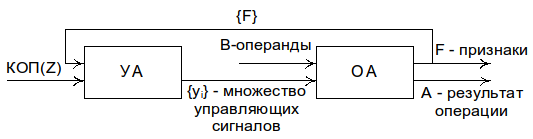
\includegraphics[scale=0.6]{images/intro.png}
	\caption{Структура цифрового автомата}
	\label{figure:intro_pic}
\end{figure}

ОА осуществляет непосредственную обработку данных путем выполнения элементарных операций над словами и выдает результат преобразования в виде двух слов: $A$ (результат) и $F$ (признаки результата, т.е. сигналы о знаках и особых значениях промежуточных и конечных результатов операций). Выполнение элементарных операций инициируется соответствующими управляющими сигналами {$y_0, y_1, y_2 ... y_m$}, которые формируются УА. 

В курсовой работе требуется разработать ОА, реализующий заданный набор арифметико-логических операций.

	%%!TEX root = main.tex
\newpage
\section{Задание}


	%\input{2.tex}
	
	%!TEX root = main.tex
\kvnoindex
\begin{figure}[H]
	\begin{subfigure}[b]{0.3\textwidth}
	\karnaughmap{4}%
	{$J^{(0)}_3:$}%
	{{$a_1$}{$a_3$}{$a_0$}{$a_2$}}%
	{x0x0xxxxx010xxxx}%
	{%
		\textcolor{Blue}{%
			\put(4, 2){\oval(1.9, 3.9)[l]}
			\put(0, 2){\oval(1.9, 3.9)[r]}
		}%
	}
	\caption{}
	\label{figure:oa10_min_J3}
	\end{subfigure}
	\qquad
	\begin{subfigure}[b]{0.3\textwidth}
	\karnaughmap{4}%
	{$K^{(0)}_3:$}%
	{{$a_1$}{$a_3$}{$a_0$}{$a_2$}}%
	{xxxx100xxxxx0x0x}%
	{%
		\textcolor{Blue}{%
			\put(4, 3.5){\oval(1.9, 0.9)[l]}
			\put(0, 3.5){\oval(1.9, 0.9)[r]}
		}%
	}
	\caption{}
	\label{figure:oa10_min_K3}
	\end{subfigure}

	\begin{subfigure}[b]{0.3\textwidth}
	\karnaughmap{4}%
	{$J^{(0)}_2:$}%
	{{$a_1$}{$a_3$}{$a_0$}{$a_2$}}%
	{xxxx1x0xxx1x0x0x}%
	{%
		\textcolor{Blue}{%
			\put(2, 3.5){\oval(3.9, 0.9)[l]}
			\put(2, 3.5){\oval(3.9, 0.9)[r]}
		}%
		\textcolor{Red}{%
			\put(1, 2){\oval(1.9, 3.9)[t]}
			\put(1, 2){\oval(1.9, 3.9)[b]}
		}%
	}
	\caption{}
	\label{figure:oa10_min_J2}
	\end{subfigure}
	\qquad
	\begin{subfigure}[b]{0.3\textwidth}
	\karnaughmap{4}%
	{$K^{(0)}_2:$}%
	{{$a_1$}{$a_3$}{$a_0$}{$a_2$}}%
	{x1x0x1xxx0x0xxxx}%
	{%
		\textcolor{Blue}{%
			\put(2, 3.5){\oval(3.9, 0.9)[l]}
			\put(2, 3.5){\oval(3.9, 0.9)[r]}
		}%
	}
	\caption{}
	\label{figure:oa10_min_K2}
	\end{subfigure}	

	\begin{subfigure}[b]{0.3\textwidth}
	\karnaughmap{4}%
	{$J^{(0)}_1:$}%
	{{$a_1$}{$a_3$}{$a_0$}{$a_2$}}%
	{x1x0110xxxxxxxxx}%
	{%
		\textcolor{Blue}{%
			\put(2, 0){\oval(3.9, 1.9)[t]}
			\put(2, 4){\oval(3.9, 1.9)[b]}
		}%
	}
	\caption{}
	\label{figure:oa10_min_J1}
	\end{subfigure}
	\qquad
	\begin{subfigure}[b]{0.3\textwidth}
	\karnaughmap{4}%
	{$K^{(0)}_1:$}%
	{{$a_1$}{$a_3$}{$a_0$}{$a_2$}}%
	{xxxxxxxxx1101x0x}%
	{%
		\textcolor{Blue}{%
			\put(2, 0){\oval(3.9, 1.9)[t]}
			\put(2, 4){\oval(3.9, 1.9)[b]}
		}%
		\textcolor{Red}{%
			\put(0.5, 2){\oval(0.9, 3.9)[t]}
			\put(0.5, 2){\oval(0.9, 3.9)[b]}
		}%
	}
	\caption{}
	\label{figure:oa10_min_K1}
	\end{subfigure}

	\begin{subfigure}[b]{0.3\textwidth}
	\karnaughmap{4}%
	{$J^{(0)}_0:$}%
	{{$a_1$}{$a_3$}{$a_0$}{$a_2$}}%
	{x1xx11xxx1xx1xxx}%
	{%
		\textcolor{Blue}{%
			\put(2, 2){\oval(3.9, 3.9)[l]}
			\put(2, 2){\oval(3.9, 3.9)[r]}
		}%
	}
	\caption{}
	\label{figure:oa10_min_J0}
	\end{subfigure}
	\qquad
	\begin{subfigure}[b]{0.3\textwidth}
	\karnaughmap{4}%
	{$K^{(0)}_0:$}%
	{{$a_1$}{$a_3$}{$a_0$}{$a_2$}}%
	{xxx1xx1xxx11xx1x}%
	{%
	{%
		\textcolor{Blue}{%
			\put(2, 2){\oval(3.9, 3.9)[l]}
			\put(2, 2){\oval(3.9, 3.9)[r]}
		}%
	}	
	}
	\caption{}
	\label{figure:oa10_min_K0}
	\end{subfigure}	
	
	\caption{Карты Карно для ФВ ОА$^{(0)}_{1}$}
	\label{figure:oa10_min_trig}
\end{figure}

\begin{figure}[H]
	\begin{subfigure}[b]{0.3\textwidth}
	\karnaughmap{4}%
	{$f^{(0)}_s:$}%
	{{$a_1$}{$a_3$}{$a_0$}{$a_2$}}%
	{x0x0011xx0101x1x}%
	{%
		{%
		\textcolor{Blue}{%
			\put(4, 1){\oval(1.9, 1.9)[l]}
			\put(0, 1){\oval(1.9, 1.9)[r]}
		}%
		\textcolor{Red}{%
			\put(3, 2){\oval(1.9, 1.9)[l]}
			\put(3, 2){\oval(1.9, 1.9)[r]}
		}%
		\textcolor{Green}{%
			\put(2.5, 2){\oval(0.9, 3.9)[t]}
			\put(2.5, 2){\oval(0.9, 3.9)[b]}
		}%
	}
	}
	\caption{}
	\label{figure:oa10_min_fs}
	\end{subfigure}
	\qquad
	\begin{subfigure}[b]{0.3\textwidth}
	\karnaughmap{4}%
	{$f^{(0)}_z:$}%
	{{$a_1$}{$a_3$}{$a_0$}{$a_2$}}%
	{x1x0000xx0000x0x}%
	{%
		{%
		\textcolor{Blue}{%
			\put(1, 3.5){\oval(1.9, 0.9)[l]}
			\put(1, 3.5){\oval(1.9, 0.9)[r]}
		}%
		}
	}
	\caption{}
	\label{figure:oa10_min_fz}
	\end{subfigure}

	\begin{subfigure}[b]{0.3\textwidth}
	\karnaughmap{4}%
	{$f_c:$}%
	{{$a_1$}{$a_3$}{$a_0$}{$a_2$}}%
	{x0x0000xx0100x0x}%
	{%
	\textcolor{Blue}{%
			\put(0.5, 2){\oval(0.9, 3.9)[t]}
			\put(0.5, 2){\oval(0.9, 3.9)[b]}
		}%
	}
	\caption{}
	\label{figure:oa10_min_fc}
	\end{subfigure}
	\qquad
	\begin{subfigure}[b]{0.3\textwidth}
	\karnaughmap{4}%
	{$f^{(0)}_p:$}%
	{{$a_1$}{$a_3$}{$a_0$}{$a_2$}}%
	{x1x0000xx1111x1x}%
	{%
		{%
		\textcolor{Blue}{%
			\put(2, 1){\oval(3.9, 1.9)[l]}
			\put(2, 1){\oval(3.9, 1.9)[r]}
		}%
		\textcolor{Red}{%
			\put(1, 0){\oval(1.9, 1.9)[t]}
			\put(1, 4){\oval(1.9, 1.9)[b]}
		}%
	}
	}
	\caption{}
	\label{figure:oa10_min_fp}
	\end{subfigure}	
	
	\begin{subfigure}[b]{0.3\textwidth}
	\karnaughmap{4}%
	{$f^{(0)}_{c'}:$}%
	{{$a_1$}{$a_3$}{$a_0$}{$a_2$}}%
	{x100110xx0x00x0x}%
	{%
		{%
		\textcolor{Blue}{%
			\put(2, 3.5){\oval(3.9, 0.9)[l]}
			\put(2, 3.5){\oval(3.9, 0.9)[r]}
		}%
	}
	}
	\caption{}
	\label{figure:oa10_min_fc1}
	\end{subfigure}

	\caption{Карты Карно для ЛФП ОА$^{(0)}_{1}$}
	\label{figure:oa10_min_flags}
\end{figure}
	%!TEX root = main.tex

\begin{figure}[H]
\begin{subfigure}[b]{0.3\textwidth}

	\karnaughmap{2}%
	{$J_i:$}%
	{{$b$}{$a$}}%
	{0x0x}%
	{%
	}
	\caption{}
	\label{oa11_J}
\end{subfigure}
\begin{subfigure}[b]{0.3\textwidth}
	\karnaughmap{2}%
	{$K_i:$}%
	{{$b$}{$a$}}%
	{x1x0}%
	{%
	\textcolor{Blue}{
		\put(1,1.5){\oval(1.9,0.9)[]}}
	}
	\caption{}
	\label{oa11_K}
\end{subfigure}
	\caption{oa11mintrig}
	\label{figure:oa11_min_trig}
\end{figure}


\begin{figure}[H]
	\begin{subfigure}[b]{0.3\textwidth}
	\karnaughmap{4}%
	{$f_s:$}%
	{{$r_1$}{$r_3$}{$r_0$}{$r_2$}}%
	{0000111100001111}%
	{%
		\textcolor{Blue}{%
			\put(3, 2){\oval(1.9, 3.9)[t]}
			\put(3, 2){\oval(1.9, 3.9)[b]}
		}%
	}
	\caption{}
	\label{figure:oa11_min_fs}
	\end{subfigure}
	\qquad
	\begin{subfigure}[b]{0.3\textwidth}
	\karnaughmap{4}%
	{$f_z:$}%
	{{$r_1$}{$r_3$}{$r_0$}{$r_2$}}%
	{1000000000000000}%
	{%
		\textcolor{Blue}{
			\put(0.5,3.5){\oval(0.9,0.9)[]}%
		}%	
	}
	\caption{}
	\label{figure:oa11_min_fz}
	\end{subfigure}

	\begin{subfigure}[b]{0.3\textwidth}
	\karnaughmap{4}%
	{$f_p:$}%
	{{$r_1$}{$r_3$}{$r_0$}{$r_2$}}%
	{1001011001101001}%
	{%
		\textcolor{Blue}{
			\put(0.5,3.5){\oval(0.9,0.9)[]}%
			\put(2.5,3.5){\oval(0.9,0.9)[]}%
			\put(1.5,2.5){\oval(0.9,0.9)[]}%
			\put(3.5,2.5){\oval(0.9,0.9)[]}%
			\put(0.5,1.5){\oval(0.9,0.9)[]}%
			\put(2.5,1.5){\oval(0.9,0.9)[]}%
			\put(1.5,0.5){\oval(0.9,0.9)[]}%
			\put(3.5,0.5){\oval(0.9,0.9)[]}%
		}%	
	}
	\caption{}
	\label{figure:oa11_min_fp}
	\end{subfigure}

	\begin{subfigure}[b]{0.3\textwidth}
	\karnaughmap{4}%
	{$f_c:$}%
	{{$r_1$}{$r_3$}{$r_0$}{$r_2$}}%
	{0000000000000000}%
	{}
	
	\caption{}
	\label{figure:oa11_min_fc}
	\end{subfigure}
	\qquad
	\begin{subfigure}[b]{0.3\textwidth}
	\karnaughmap{4}%
	{$f'_c:$}%
	{{$r_1$}{$r_3$}{$r_0$}{$r_2$}}%
	{0000000000000000}%
	{}


	\caption{}
	\label{figure:oa11_min_fc1}
	\end{subfigure}


	\caption{oa11minflags}
	\label{figure:oa11_min_flag}

\end{figure}

	%%!TEX root = main.tex

\newpage
%\section*{ЗАКЛЮЧЕНИЕ}
%\addcontentsline{toc}{section}{ЗАКЛЮЧЕНИЕ}
\begin{center}
\textbf{ЗАКЛЮЧЕНИЕ}
\end{center}
\addcontentsline{toc}{section}{ЗАКЛЮЧЕНИЕ}


	%%!TEX root = main.tex

\newpage

\begin{center}
\textbf{БИБЛИОГРАФИЧЕСКИЙ СПИСОК}
\end{center}
\addcontentsline{toc}{section}{БИБЛИОГРАФИЧЕСКИЙ СПИСОК}


\end{document}